\documentclass[10pt,twocolumn]{article}
\setlength\textwidth{6.875in}
\setlength\textheight{8.875in}
% set both margins to 2.5 pc
\setlength{\oddsidemargin}{-0.1875in}% 1 - (8.5 - 6.875)/2
\setlength{\evensidemargin}{-0.1875in}
\setlength{\marginparwidth}{0pc}
\setlength{\marginparsep}{0pc}%
\setlength{\topmargin}{0in} \setlength{\headheight}{0pt}
\setlength{\headsep}{0pt}
\setlength{\footskip}{37pt}%
\setlength{\columnsep}{0.3125in}
\setlength{\columnwidth}{3.28125in}% (6.875 - 0.3125)/2 = 3.28125in
\setlength{\parindent}{1pc}
\newcommand{\myMargin}{1.00in}
\usepackage[top=\myMargin, left=\myMargin, right=\myMargin, bottom=\myMargin, nohead]{geometry}
\usepackage{epsfig,graphicx}
\usepackage{palatino}
\usepackage{fancybox}
\usepackage[procnames]{listings}
\usepackage{hyperref}

\newenvironment{commentary}
{ \vspace{-0.1in}
  \begin{quotation}
  \noindent
  \small \em
  \rule{\linewidth}{1pt}\\
}
{
  \end{quotation}
}

\title{Advanced Parameterization Manual}
\author{Adam Izraelevitz \\
EECS Department, UC Berkeley\\
{\tt  adamiz@eecs.berkeley.edu}
}
\date{\today}

\newenvironment{example}{\VerbatimEnvironment\begin{footnotesize}\begin{Verbatim}}{\end{Verbatim}\end{footnotesize}}
\newcommand{\kode}[1]{\begin{footnotesize}{\tt #1}\end{footnotesize}}

\def\code#1{{\small\tt #1}}

\def\note#1{\noindent{\bf [Note: #1]}}
%\def\note#1{}

% "define" Scala
\usepackage[T1]{fontenc}  
\usepackage[scaled=0.82]{beramono}  
\usepackage{microtype} 

\sbox0{\small\ttfamily A}
\edef\mybasewidth{\the\wd0 }

\lstdefinelanguage{scala}{
  morekeywords={abstract,case,catch,class,def,%
    do,else,extends,false,final,finally,%
    for,if,implicit,import,match,mixin,%
    new,null,object,override,package,%
    private,protected,requires,return,sealed,%
    super,this,throw,trait,true,try,%
    type,val,var,while,with,yield},
  sensitive=true,
  morecomment=[l]{//},
  morecomment=[n]{/*}{*/},
  morestring=[b]",
  morestring=[b]',
  morestring=[b]"""
}

\usepackage{color}
\definecolor{dkgreen}{rgb}{0,0.6,0}
\definecolor{gray}{rgb}{0.5,0.5,0.5}
\definecolor{mauve}{rgb}{0.58,0,0.82}

% Default settings for code listings
\lstset{language=scala,
  showstringspaces=false,
  columns=fixed, % basewidth=\mybasewidth,
  basicstyle={\small\ttfamily},
  numbers=none,
  numberstyle=\footnotesize\color{gray},
  % identifierstyle=\color{red},
  keywordstyle=\color{blue},
  commentstyle=\color{dkgreen},
  stringstyle=\color{mauve},
  breakatwhitespace=true,
  procnamekeys={def, val, var, class, trait, object, extends},
  procnamestyle=\ttfamily\color{red},
}

\lstnewenvironment{scala}
{\lstset{language=scala}}
{}
\lstnewenvironment{cpp}
{\lstset{language=C++}}
{}
\lstnewenvironment{bash}
{\lstset{language=bash}}
{}
\lstnewenvironment{verilog}
{\lstset{language=verilog}}
{}

\newcommand{\isc}{
\lstinline
}

\lstdefinestyle{scala}{language=scala,
  showstringspaces=false,
  columns=fixed, % basewidth=\mybasewidth,
  basicstyle={\small\ttfamily},
  numbers=none,
  numberstyle=\footnotesize\color{gray},
  % identifierstyle=\color{red},
  keywordstyle=\color{blue},
  commentstyle=\color{dkgreen},
  stringstyle=\color{mauve},
  breakatwhitespace=true,
  procnamekeys={def, val, var, class, trait, object, extends},
  procnamestyle=\ttfamily\color{red},
}


\lstset{frame=, basicstyle={\footnotesize\ttfamily}}

\lstset{frame=}

\begin{document}
\maketitle{}


\section{Introduction}

This document is a manual for using the advanced parameter library within {\em Chisel}. For more general information regarding {\em Chisel} as a hardware construction language, please see the Getting Started documentation.

As hardware designs grow in complexity, modularity becomes necessary for maintaince and verification. The primary use case for {\em Chisel} is describing diverse and highly-parameterized hardware generators, and we quickly realized that the traditional parameterization method forces brittleness into a design's source code and limits component reuse.

The outline of this document is as follows: in Section \ref{sec:advanced}, we describe the basic objects and methods for the advanced parameterization mechanism, as well as the required boilerplate to use it. In Section \ref{sec:examples}, a series of increasingly complex examples of design patterns are described. For each example, we propose the simplest parameterization scheme which solves the problem. As the examples build in complexity, so do the parameterization requirements, until we we arrive at the described advanced parameterization mechanism. The next section, Section \ref{sec:knobs}, introduces the concept of \code{Knobs} and their relationship to design constraints and the \code{Parameters} object. Finally, in Section \ref{sec:heuristics}, we explain multiple design heuristics which should be followed when using advanced parameterization.

\section{Advanced Parameterization}
\label{sec:advanced}
	
Every {\em Chisel} Module has a member \code{params} of class \code{Parameters} that provides the mechanism for passing parameters between modules.

This section describes the following features: (1) the \code{Parameters} class and associated methods/members; (2) the basic usage model; (3) syntactic sugar; (4) boilerplate code for exposing parameters to external users/programs; (5) advanced functionality via Views (site, here, up).

\subsection{Classes and Methods}
The \code{Parameters} class has the following base methods:

  \begin{scala}
class Parameters {
  // returns a value of type T
  def apply[T](key:Any):T 
  
  // returns new Parameters class
  def alter(mask:(Any,View,View,View)=>Any):Parameters 
  
  // returns a Module's Parameters instance
  def params:Parameters
}
  \end{scala}
\code{View} is a class containing a base method:
  \begin{scala}
class View {
  // returns a value of type T
  def apply[T](key:Any):T 
}
  \end{scala}
\code{Parameters} has a factory object containing one basic method:
  \begin{scala}
object Parameters {
  // returns an empty Parameters instance
  def empty:Parameters
}
  \end{scala}

The \code{Module} factory object now has an additional apply method:
  \begin{scala}
object Module {
  // returns a new Module of type T, initialized with a Parameters instance if  _p !=None.
  def apply[T<:Module](c: =>T)(implicit _p: Option[Parameters] = None):T
}
  \end{scala}

\subsection{Basic Usage Model}

This example shows the simplest usage of (1) quering params, (2) altering a Parameters object, and (3) passing a Parameters object to a Module:

\begin{scala}
class Tile extends Module { 
  val width = params[Int]('width') 
}
object Top {
  val parameters = Parameters.empty
  val tile_parameters = parameters.alter( (key,site,here,up) => {
    case 'width' => 64
  })
  def main(args:Array[String]) = {
    chiselMain(args,()=>Module(new Tile)(Some(tile_parameters)))
  }
}
\end{scala}

Within the Module \code{Tile}, the \code{params} member is queried by calling Parameters.apply with the key and return value type.

In \code{Top}, an empty parameters is created by calling Parameters.empty; then it is altered with a function of type \code{(Any,View,View,View) => Any} to return a new Parameters instance, which is assigned to \code{tile\_parameters}. 

After wrapping \code{tile\_parameters} within \code{Some:Option[Parameters]}, it is passed as a second argument to the Module object when passed to \code{chiselMain}.

\subsection{Syntactic Sugar: Field[T]}

The simple example requires the return type \code{Int} must be included as an argument to the apply method, otherwise the Scala compiler will throw an error:

\begin{scala}
class Tile extends Module { 
  val width = params[Int]('width') 
}
\end{scala}

Alternatively, one can create a case object for each key which extends \code{Field[T]} and pass that directly into \code{params} apply method. Because \code{Field} contains the return type information, the type does not need to be passed:

\begin{scala}
case object Width extends Field[Int]
class Tile extends Module { 
  val width = params(Width) 
}
\end{scala}

For the rest of the document, assume the key to every query is a case class that extends \code{Field[T]} with the correct return type.

\subsection{Syntactic Sugar: Passing and Altering}

\begin{figure}[h]
\centering
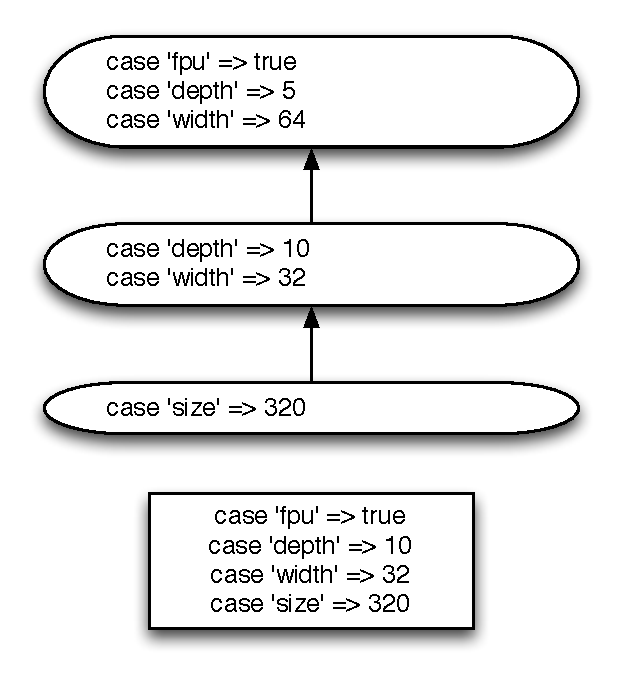
\includegraphics[width=3in]{figs/alter}
\caption{An example of Memory's key/value chain and flat map.}
\label{fig:alter}
\end{figure}

As a module hierarchy is formed, \code{Parameters} objects are passed between a parent module and a child module. If specified by the programmer, these objects can be copied and altered prior to instantiating the child.

Anytime an alteration is performed, {\em Chisel} internally copies the existing chain of key/value mappings and attaches the provided key/value mappings to the bottom of this chain. When a query is evaluated, it first queries the chain's bottom key/value mapping. If there is no match, the query is then evaluated on the next key/value mapping in the chain, and so forth. If a query reaches the top of the chain with no matches, {\em Chisel} triggers a \code{ParameterUndefinedException}.

When instantiating a child, the parent can pass its \code{Parameters} object one of two ways:
\begin{enumerate}
  \item Explicitly pass its \code{Parameters} object to its child via a second argument to the Module factory, wrapped in \code{Option[Parameters]}:
\begin{scala}
class Tile extends Module { 
  val width = params(Width) 
  val core = Module(new Core)(Some(params))
  // Explicit passing of Tile's params to Core
}
\end{scala}
  \item Implicitly pass its \code{Parameters} object to its child:
\begin{scala}
class Tile extends Module { 
  val width = params(Width)
  val core = Module(new Core)
  // Implicit passing of Tile's params to Core
}
\end{scala}
\end{enumerate}

If a parent wants to copy/alter the child's dictionary, the parent has two methods to do so:
\begin{enumerate}
  \item Provide a PartialFunction mapping as an argument to the Module factory. Internally, {\em Chisel} will copy the parent's \code{Parameters} object and apply the alteration:
\begin{scala}
class Tile extends Module { 
  val width = params(Width)
  val core = Module(new Core,{case Width => 32})
  // Provide PartialFunction to Module factory constructor to alter Core's \code{Parameters} object
}
\end{scala}
  \item Call the \code{Parameter.alter} function, which returns a new \code{Parameters} object. This approach gives the programmer access to the new \code{Parameters} object, as well as the ability to use \code{site}, \code{here}, and \code{up} (see Sections \ref{sec::site}, \ref{sec::here}, \ref{sec::up}) :
\begin{scala}
class Tile extends Module { 
  val width = params(Width)
  val core_params = params.alter(
    (pname,site,here,up) => pname match {
      case Width => 32
    })
  val core = Module(new Core)(Some(core_params))
  // Use the Parameter.alter method to return an altered Parameter object. Only use when site, here, or up mechanisms are needed
}
\end{scala}
\end{enumerate}
A more complicated example of a alteration chain is shown in Figure \ref{fig:alter} and describe below:
\begin{scala}
class Tile extends Module { 
  ...
  val core = Module(new Core, {case FPU => true; case QDepth => 20; case Width => 64})
}
class Core extends Module {
  val fpu = params(FPU)
  val width = params(Width)
  val depth = params(Depth)
  val queue = Module(new Queue,{case Depth => depth*2; case Width => 32})
}
class Queue extends Module {
  val depth = params(Depth)
  val width = params(Width)
  val mem = Module(new Memory,{case Size => depth * width})
}
class Memory extends Module {
  val size = params(Size)
  val width = params(Width)
}
\end{scala}

\subsection{ChiselConfig and Boilerplate}
\label{sec::config}

{\em Chisel}'s mechanism to seed the top-level parameters is through a \code{ChiselConfig} object. \code{ChiselConfig.topDefinitions} contains the highest parameter definitions and is of the following form:
\begin{scala}
case object Width extends Field[Int]
class DefaultConfig extends ChiselConfig { 
  val topDefinitions:World.TopDefs = {
    (pname,site,here) => pname match {
      case Width => 32
    }
  }
}
\end{scala}
Normally, a design calls \code{chiselMain.apply} to instantiate a design. To use {\em Chisel}'s parameterization mechanism and correctly seed a \code{ChiselConfig}, one should instead call \code{chiselMain.run} with the design NOT surrounded by the \code{Module} factory. The reason for this change is to preserve backwards compatibility with existing designs, although we intend to fix this in future releases. 

An example of calling \code{chiselMain.run} is as follows:
\begin{scala}
object Run { 
  def main(args: Array[String]): Unit = {
    chiselMain.run(args, () => new Tile())
  }
}
\end{scala}
To instantiate a design with a specific \code{ChiselConfig}, simply call the {\em Chisel} compiler with the \code{-{-}configInstance {\it project\_name.configClass\_name}} argument.

\subsection{Using site}
\label{sec::site}

\begin{figure*}
\begin{center}
\begin{tabular}{cc}
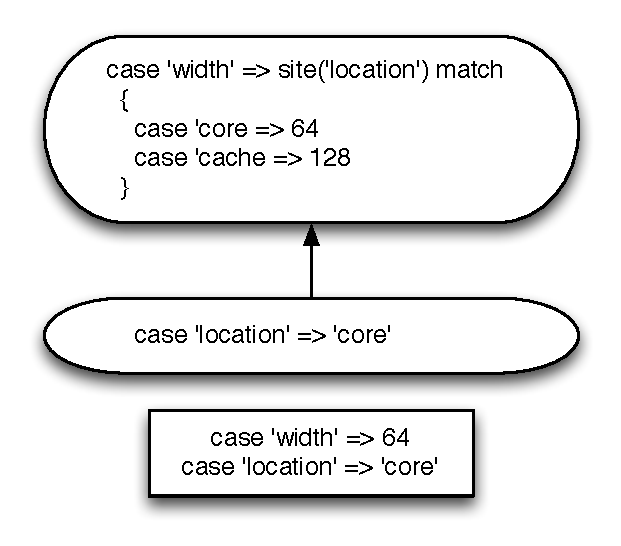
\includegraphics[height=2.0in]{figs/sitea} &
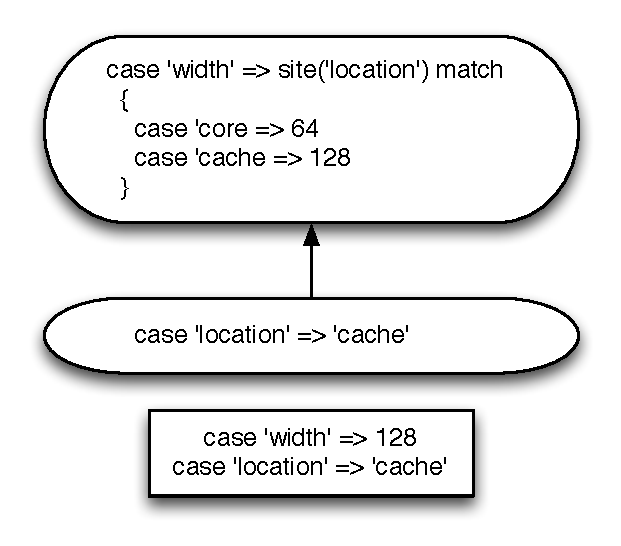
\includegraphics[height=2.0in]{figs/siteb} \\
(a) Core's key/value chain and flat map & (b) Cache's key/value chain and flat map \\
\end{tabular}
\end{center}
\caption{For (a), site(Location) will return Core, while in (b) site(Location) will return Cache.}
\label{fig:site}
\end{figure*}
To help the designer express dependencies between parameters, we added the \code{site} mechanism. To understand its function, remember that conceptually, a queried Module's params member first looks at the bottom key/value mapping in its chain of key/value mappings. If there is no match, the query moves up the chain. 

Suppose we have some modules which have following form:

\begin{scala}
class Core extends Module {
  val data_width = params(Width)
  ...
}
class Cache extends Module {
  val line_width = params(Width)
  ...
}
\end{scala}
Unfortunately, both have identical queries for \code{Width} but, for this example's sake, have different semantic meaning. Inside a core, \code{Width} means the word size, while in the \code{Cache}, \code{Width} means the width of a cache line. We want to be able to easily tailor the parameter's response to either query.

The \code{site} mechanism allows a key/value mapping in the middle of the chain to make its own queries that start at the bottom of the chain.

Consider the following example:
\begin{scala}
class DefaultConfig extends ChiselConfig { 
  val top:World.TopDefs = {
    (pname,site,here) => pname match {
       case Width => site(Location) match {
         case 'core' => 64 // data width
         case 'cache' => 128  // cache line width
       }
    }
  }
}
class Tile extends Module { 
  val core = Module(new Core, {case Location => 'core'})
  val cache = Module(new Cache, {case Location => 'cache'})
}
\end{scala}
The top-level key/value mapping is using \code{site} to query the bottom of the chain for \code{Location}. Depending on what value returns (either \code{'core'} or \code{'cache'}), the top-level key/value mapping produces a different value (Figure \ref{fig:site}).

\subsection{Using here}
\label{sec::here}

\begin{figure}[h]
\centering
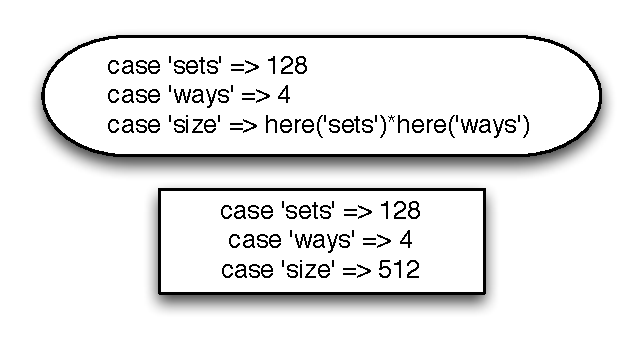
\includegraphics[width=3in]{figs/here}
\caption{Instead of using 128 or 4 directly, we can access it via here(Sets) and here(Ways), respectively.}
\label{fig:alter}
\end{figure}

If a parameter is a deterministic function of other parameters expressed at the same group in the key/value mapping chain, one does not want to duplicate a value, as giving a new value would require multiple changes. Instead, one can use the \code{here} mechanism to query the same group of key/value mappings that \code{here} was called:

\begin{scala}
class Tile extends Module { 
  val cache_params = params.alter(
    (pname, site, here, up) => pname match {
      case Sets => 128
      case Ways => 4
      case Size => here(Sets)*here(Ways)
    })
  val cache = Module(new Cache)(cache_params)
}
\end{scala}

\subsection{Using up}
\label{sec::up}

The \code{up} mechanism enables the user to query the parent group of key/value mappings. It is equivalent to calling \code{Parameters.apply} directly, but can be done within calling \code{Parameters.alter}. For an example use, see Section \ref{sec::rename}.

\section{Examples}
\label{sec:examples}

The three goals of any parameterization scheme are: (1) all searchable parameters are exposed at the top level; (2) source code must never change when evaluating different points; (3) adding new parameters requires little source code change. After each example is described, we present the simplest parameterization scheme that supports the desired design space without violating any of the three goals. As examples grow in complexity, so too must the simplest parameterization scheme, until we arrive at the current advanced parameterization method.

\subsection{Simple Parameters}

\begin{figure}[h]
\centering
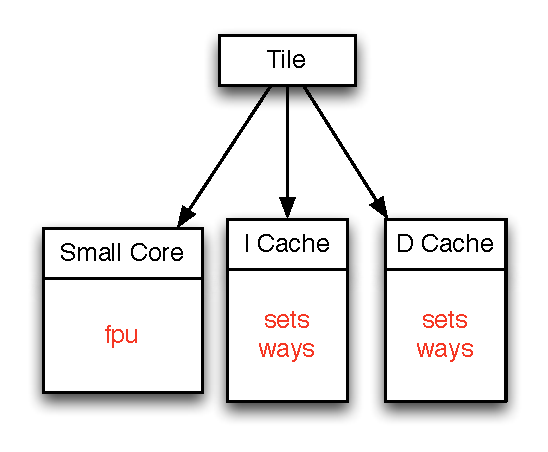
\includegraphics[width=3in]{figs/ex1}
\caption{For a few number of parameters, the simplest scheme is to pass them directly via constructor arguments.}
\label{fig:ex1}
\end{figure}

In this simple design, we only vary core and cache-specific parameters. The most straightforward parameterization scheme is passing all parameters via arguments to \code{Tile}'s constructor. These values are then passed to \code{Core} and \code{Cache} via their respective constructors: 

\begin{scala}
class Tile (val fpu:Boolean, val ic_sets:Int, val ic_ways:Int, val dc_sets:Int, val dc_ways:Int) extends Module { 
  val core = Module(new Core(fpu))
  val icache = Module(new Cache(ic_sets,ic_ways)
  val dcache = Module(new Cache(dc_sets,dc_ways))
  ... 
}
class Core (val fpu:Boolean) {...}
class Cache(val sets:Int, val ways:Int) extends Module {...}
\end{scala}

No source code changes are necessary to explore our parameter space, and all searchable parameters are exposed at the top. In addition, adding a new parameter, because this example is simple, requires very few changes to our source code.

\subsection{Disjoint Parameter Sets}

\begin{figure}[h]
\centering
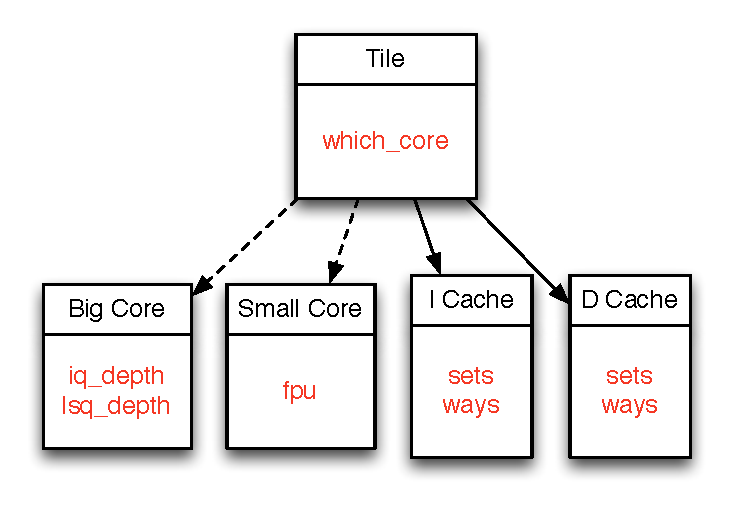
\includegraphics[width=3in]{figs/ex2}
\caption{For disjoint parameter sets, we can group sets of parameters into configuration objects to pass as constructor arguments.}
\label{fig:ex2}
\end{figure}

In this next design, we are designing a chip which could instantiate different cores, each with its own set of parameters. If we apply our simple solution, the number of arguments to \code{Tile}'s constructor would be huge as it must contain all parameters for all possible cores (which would likely be much greater than two cores!).

One could propose that a better solution would be to group parameters into configuration objects. For example, we could group all \code{BigCore} parameters into a \code{BigCoreConfig} case class, and all \code{SmallCore} parameters into a \code{SmallCoreConfig} class, both of which extend \code{CoreConfig}. In addition, we have our caches and \code{Tile} accept a \code{CacheConfig} and \code{TileConfig}, respectively, within their constructors.

\begin{scala}
abstract class CoreConfig {}
case class BigCoreConfig(iq_depth:Int, lsq_depth:Int) extends CoreConfig
case class SmallCoreConfig(fpu:Boolean) extends CoreConfig
case class CacheConfig(sets:Int, ways:Int)
case class TileConfig(cc:CoreConfig, icc:CacheConfig, dcc:CacheConfig)

class Tile (val tc:TileConfig) extends Module { 
  val core = tc.cc match {
    case bcc:BigCoreConfig => Module(new BigCore(tc.bcc))
    case scc:SmallCoreConfig => Module(new SmallCore(tc.scc))
  }
  val icache = Module(new Cache(tc.icc)
  val dcache = Module(new Cache(tc.dcc))
  ... 
}
...
\end{scala}
  
\subsection{Location-Independent Parameters}

\begin{figure}[h]
\centering
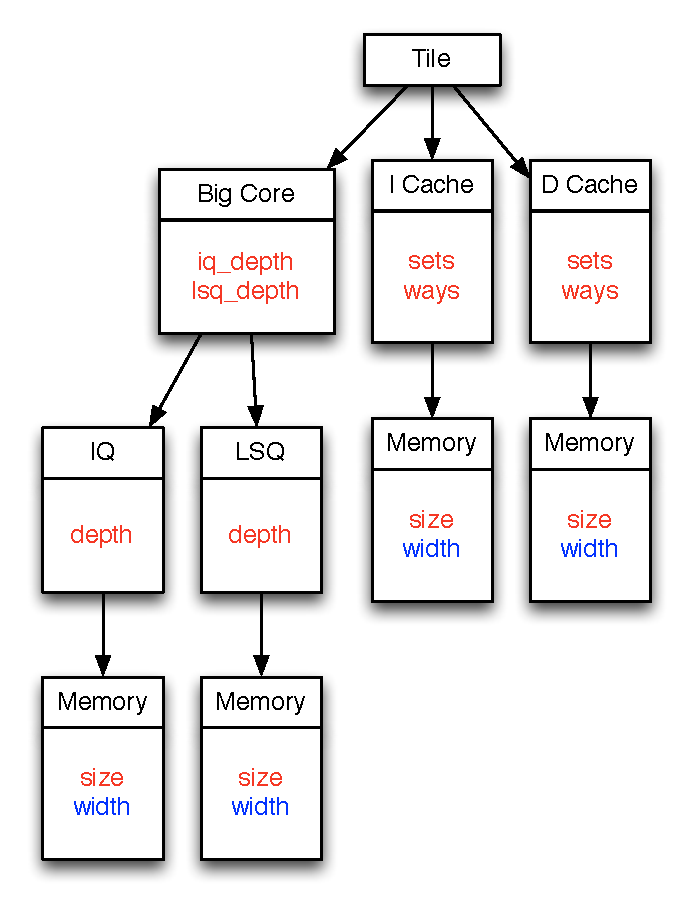
\includegraphics[width=3in]{figs/ex3}
\caption{For location-independent parameters, every module has a parameter dictionary, which they can copy and alter before passing to each child module.}
\label{fig:ex3}
\end{figure}

The subtle reason why nested configuration objects are extremely brittle is the structure of the nested configuration objects encodes the module hierarchy. Given a new design described in Figure \ref{fig:ex3}, we assume that \code{BigCore}'s IQ and LSQ, as well as the icache and dcache, instantiate a \code{Memory} module. This Memory module contains a \code{width} parameter, and in order for the design to function correctly, all of Memory widths must be set to the same value. To ensure this requirement, the follow code might be written:

\begin{scala}
case class MemConfig(size:Int, banks:Int, width:Int)
case class CacheConfig(sets:Int, ways:Int, mc:MemConfig)
case class QueueConfig(depth:Int, mc:MemConfig)
case class BigCoreConfig(iqc:QueueConfig, lsqc:QueueConfig, mc:MemConfig)

case class TileConfig(cc:CoreConfig, icc:CacheConfig, dcc:CacheConfig)

class Tile (val tc:TileConfig) extends Module { 
  val core = tc.cc match {
    case bcc:BigCoreConfig => Module(new BigCore(tc.bcc))
    case scc:SmallCoreConfig => Module(new SmallCore(tc.scc))
  }
  val icache = Module(new Cache(tc.icc)
  val dcache = Module(new Cache(tc.dcc))
  
  require(tc.dcc.mc.width == tc.icc.mc.width)
  require(tc.bcc.iqc.mc.width == tc.bcc.lsqc.mc.width)
  require(tc.dcc.mc.width == tc.bcc.lsqc.mc.width)
  ...
}
...
\end{scala}

The series of require statements is extremely brittle, as any change in our design's hierarchy requires massive rewrites of all of these statements. Omitting the require statements is not a viable option; these statements are necessary to enforce this fundamental design requirement.

This flaw in configuration objects leads us towards the first functionality of our custom parameterization solution, namely a copy/alter dictionary of type \code{Parameters}. We use this key-value structure (map or dictionary) to store a module's parameters.

To parameterize the design in Figure \ref{fig:ex3}, we implicitly pass the \code{Parameters} object and, if an alter is needed, provide a \code{PartialFunction} to the \code{Module} factory. Recall from Section \ref{sec:advanced} that the class \code{MyConfig} (extends \code{ChiselConfig}) must be passed to the {\em Chisel} compiler via the \code{-{-}configInstance} flag to seed the top-level parameters:
\begin{scala}
class DefaultConfig() extends ChiselConfig {
  val top:World.TopDefs = {
    (pname,site,here) => pname match {
      case IQ_depth => 10
      case LSQ_depth =>10
      case Ic_sets => 128
      case Ic_ways => 2
      case Dc_sets => 512
      case Dc_ways => 4
      case Width => 64
      // since any module querying Width should return 64, the name should NOT be unique to modules
    }
  }
}
class Tile extends Module { 
  val core = Module(new Core)(params)
  val ic_sets = params(Ic_sets)
  val ic_ways = params(Ic_ways)
  val icache = Module(new Cache, {case Sets => ic_sets; case Ways => ic_ways})
  // we can rename Ic_sets to Sets, effectively isolating Cache's query keys from any design hierarchy dependence
  val dc_sets = params(Dc_sets)
  val dc_ways = params(Dc_ways)
  val dcache = Module(new Cache, {case Sets => dc_sets; case Ways => dc_ways})
  // similarly we rename Dc_sets to Sets and Dc_ways to Ways
}
class Core extends Module {
  val iqdepth = params(IQ_depth)
  val iq = Module(new Queue, {case Depth => iqdepth})
  val lsqdepth = params(LSQ_depth)
  val lsq = Module(new Queue, {case Depth => lsqdepth})
  ...
}
class Queue extends Module {
  val depth = params(Depth)
  val mem = Module(new Memory,{case Size => depth})
  ...
}
class Cache extends Module {
  val sets = params(Sets)
  val ways = params(Ways)
  val mem = Module(new Memory,{case Size => sets*ways})
}
class Memory extends Module {
  val size = params(Size)
  val width = params(Width)
}
\end{scala}

Although this parameterization method is reasonably verbose, it scales well with adding parameters, requires no source changes, and allows a single parameter, such as \code{Width}, to change all leaf modules.

\subsection{Location-Specific Parameters}

\begin{figure}[h]
\centering
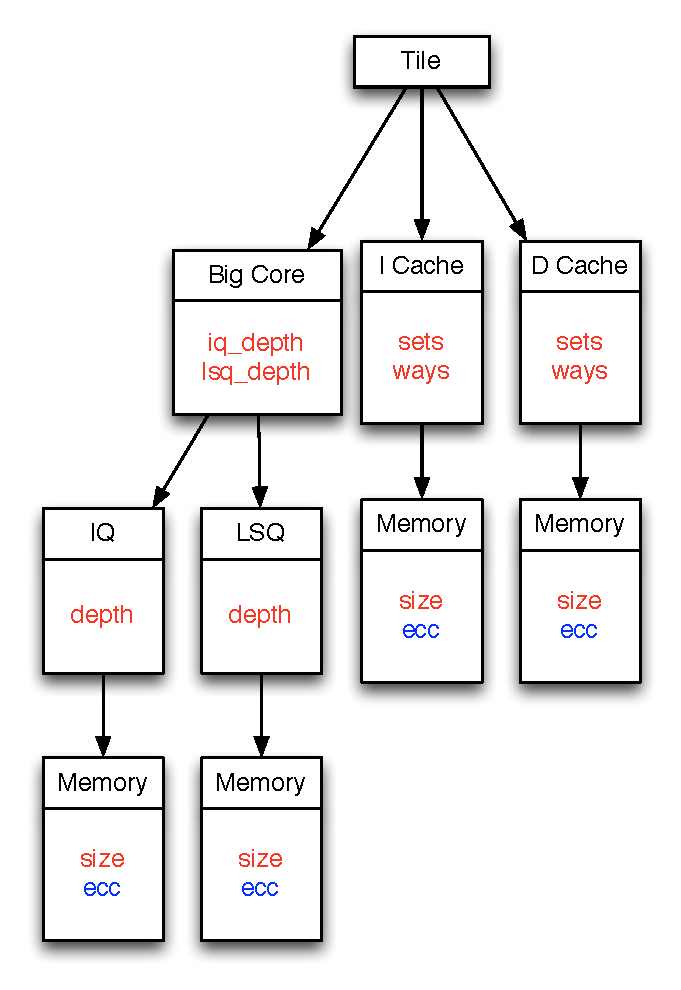
\includegraphics[width=3in]{figs/ex4}
\caption{For location-dependent parameters, we can use the \code{site} mechanism to customize these parameters at the top level.}
\label{fig:ex4}
\end{figure}

As we saw in the previous section, copying and altering a \code{Parameters} object can be verbose. If we wanted to add an ECC parameter to our \code{Memory} module, which depends on where the \code{Memory} is instantiated, we would change source code in multiple parents to rename each parameter (e.g. ECC\_icache => ECC).

In the example depicted in Figure \ref{fig:ex4}, we instead use the \code{site} functionality of our \code{Parameters} object to obtain location-specific information, and tailor the value we return to that location-specific value. After adding the location-specific information, we drastically reduce the amount of code changes necessary:

\begin{scala}
class DefaultConfig() extends ChiselConfig {
  val top:World.TopDefs = {
    (pname,site,here) => pname match {
      case Depth => site(Queue_type) match {
        case 'iq' => 20
        case 'lsq' => 10
      }
      case Sets => site(Cache_type) match {
        case 'i' => 128
        case 'd' => 512
      }
      case Ways => site(Cache_type) match {
        case 'i' => 2
        case 'd' => 4
      }
      case Width => 64
      // since any module querying Width should return 64, the name should NOT be unique to modules
      case ECC => site(Location) match {
        'incore' => false
        'incache' => true
      }
    }
  }
}
class Tile (val params:Parameters) extends Module { 
  val core = Module(new Core,{Location => 'incore'})
  // we can give core and its child modules a location identifier
  
  val cacheparams = params.alter({Location => 'incache'})
  // we can give both caches and all their child modules a location identifier
  val icache = Module(new ICache)(cacheparams)
  val dcache = Module(new DCache)(cacheparams)
}
class Core extends Module {
  val iq = Module(new IQ)
  val lsq = Module(new LSQ)
  ...
}
class IQ extends Module {
  val depth = params(Depth)
  val mem = Module(new Memory, {Size = depth})
  // in some cases, using copy/alter is preferred instead of \code{site} (see Design Heuristics for more details)
  ...
}
class LSQ extends Module {
  val depth = params(Depth)
  val mem = Module(new Memory, {Size = depth})
  ...
}
class ICache extends Module {
  val sets = params(Sets)
  val ways = params(Ways)
  val mem = Module(new Memory,{Size => sets*ways})
}
class DCache extends Module {
  val sets = params(Sets)
  val ways = params(Ways)
  val mem = Module(new Memory, {Size => sets*ways})
}
class Memory extends Module {
  val size = params(Size)
  val ecc = params(ECC)
}
\end{scala}

\subsection{Derivative Parameters}

\begin{figure}[h]
\centering
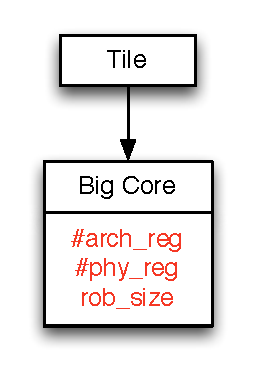
\includegraphics[width=1.5in]{figs/ex5}
\caption{To derive a parameter from another top-level parameter, we can use the here functionality to avoid duplicating a parameter value.}
\label{fig:ex5}
\end{figure}

In Figure \ref{fig:ex5}, we always want our ROB to be four-thirds the size of the difference between the number physical registers and the number of architectural registers. If we express this in \code{MyConfig.top}, it could look like the following:

\begin{scala}
case object NUM_arch_reg extends Field[Int]
case object NUM_phy_reg extends Field[Int]
case object ROB_size extends Field[Int]
class DefaultConfig() extends ChiselConfig {
  val top:World.TopDefs = {
    (pname,site,here) => pname match {
      case NUM_arch_reg => 32
      case NUM_phy_reg => 64
      case ROB_size => 4*(64-32)/3
  }
}
\end{scala}
However, if we later increase the number of physical registers, we need to remember to update the value in the derivation of the ROB size. To avoid this potential error, one should use the 'here' functionality to query the same group of parameters:

\begin{scala}
class DefaultConfig() extends ChiselConfig {
  val top:World.TopDefs = {
    (pname,site,here) => pname match {
      case NUM_arch_reg => 32
      case NUM_phy_reg => 64
      case ROB_size => 4*(here(NUM_phy_reg) - here(NUM_arch_reg))/3
  }
}
\end{scala}

\subsection{Renaming Parameters}
\label{sec::rename}

\begin{figure}[h]
\centering
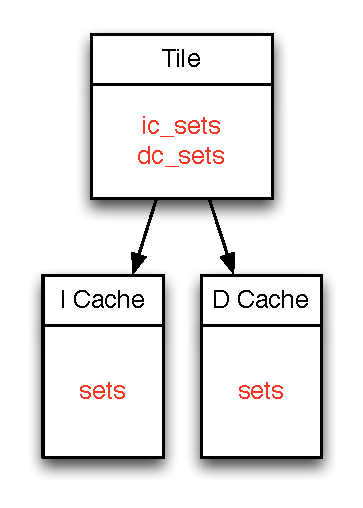
\includegraphics[width=1.5in]{figs/ex6}
\caption{To rename or programmatically alter a parameter based on the previous value, one can use the up mechanism to query the parent's \code{Parameters} object.}
\label{fig:ex6}
\end{figure}

In Figure \ref{fig:ex6}, both cache modules query for a \code{sets} parameter. However, \code{Tile} has \code{ic\_sets} and \code{dc\_sets} as parameters. To rename the parameters, we can read the parent value and alter the child's \code{Parameters} object:

\begin{scala}
class Tile extends Module {
  val ic_sets = params(Ic_sets)
  val ic = Module(new Cache,{case Sets => ic_sets})
  val dc_sets = params(Ic_sets)
  val dc = Module(new Cache,{case Sets => dc_sets})
    ...
}
\end{scala}
Alternatively, we can use the 'up' mechanism within the Parameters.alter method to query the parent module's Parameter object:
\begin{scala}
class Tile extends Module {
  val ic_params = params.alter(
    (pname,site,here,up) => pname match {
      case Sets => up(Ic_sets)
    }
  )
  val ic = Module(new Cache)(ic_params)
  ...
}
\end{scala}
In general one should never use the \code{up} mechanism as it is more verbose. However, it can be useful if the parent is making significant changes to a child's \code{Parameters} object, as all changes can be contained the \code{Parameter.alter} method because one has access to all three central mechanisms (\code{up}, \code{site}, and \code{here}).

\section{External Interface}
\label{sec:knobs}

So far, this document has only describe mechanisms to manipulate parameters at a top-level class (\code{ChiselConfig}). However, to actually generate multiple C++ or Verilog designs, we need to manually change these parameters.

One would prefer to express design constraints (parameter ranges, dependencies, constraints) and leave the actual instantiation of a specific design separate from the expression of the valid design space.

With that motivation, {\em Chisel} has an additional feature based around the concept of ``Knobs,'' or parameters that are created specifically to explore a design space. This section will describe Knobs and their uses, the Dump Object, adding constraints to parameters/Knobs, and the two modes to running the Chisel compiler: --configCollect and --configInstance.

\subsection{Knobs}
A generator has some parameters that are fixed, and others that dictate the specific design point being generated. These generator-level parameters, called Knobs, have an additional key-value mapping to allow external programs and users to easily overwrite their values.

Knobs can only be instantiated within a \code{ChiselConfig} subclass's \code{topDefinitions}:

\begin{scala}
package example
class MyConfig extends ChiselConfig {
  val topDefinitions:World.TopDefs = {
    (pname,site,here) => pname match {
      case NTiles => Knob('NTILES')
      case .... => .... // other non-generator parameters go here
    }
  }
  override val knobValues:Any=>Any = {
    case 'NTILES' => 1 // generator parameter assignment
  }
}
\end{scala}

When the query \code{NTiles} matches within topDefinitions, the \code{Knob('NTILES')} is returned. Internally, Chisel will lookup \code{'NTILES'} within MyConfig.knobValues and return 1. As described in Section \ref{sec::config}, the flag required to execute a generator with this specific config is:

\code{sbt run ... -{-}configInstance example.MyConfig}

Suppose we wanted to instantiate a new design that had two tiles: simply use Scala's class inheritance and overwrite the knobValues method:

\begin{scala}
package example
class MyConfig2 extends MyConfig {
  override val knobValues:Any=>Any = {
    case 'NTILES' => 2 // will generate new design with 2 tiles
  }
}
\end{scala}

Notice that both classes can exist in the source code, so both designs can be instantiated from the commandline. For the new design with two tiles, simply call:

\code{sbt run ... -{-}configInstance example.MyConfig2}

\subsection{Dump}

Downstream from Chisel, other tools might need to know specific parameter/Knob assignments. If so, just pass the Knob/value to the Dump object, which will write the name and value to a file, then return the Knob/value:

\begin{scala}
package example
class MyConfig extends ChiselConfig {
  val topDefinitions:World.TopDefs = {
    (pname,site,here) => pname match {
      case Width => Dump('Width',64) // will return 64. Requires naming the parameter as the 1st argument
      case NTiles => Dump(Knob('NTILES')) // will return Knob('NTILES'), no name needed
    }
  }
  override val knobValues:Any=>Any = {
    case 'NTILES' => 1 // generator parameter assignment
  }
}
\end{scala}

The name and value of each dumped parameter will be written to a \code{*.knb} file located in the directory set by \code{-{-}targetDir {\it path}}.

\subsection{Constraints}

Now that external programs/users can easily overwrite a configuration's \code{knobValue} method, we have provided a mechanism for defining legal ranges for Knobs. Within a \code{ChiselConfig}, one can overwrite another method called \code{topConstraints}:

\begin{scala}
package example
class MyConfig extends ChiselConfig {
  val topDefinitions:World.TopDefs = {
    (pname,site,here) => pname match {
      case NTiles => Knob('NTILES')
    }
  }
  override val topConstraints:List[ViewSym=>Ex[Boolean]] 
    = List( { ex => ex(NTiles) >  0 },
            { ex => ex(NTiles) <= 4 })
  override val knobValues:Any=>Any = {
    case 'NTILES' => 1 // generator parameter assignment
  }
}
\end{scala}

Now, if someone tried to instantiate our design with the following configuration and command, it would fail:

\begin{scala}
package example
class BadConfig extends ChiselConfig {
  override val knobValues:Any=>Any = {
    case 'NTILES' => 5 // would violate our constraint, throws an error
  }
}

// throws 'Constriant failed' error
sbt run ... --configInstance example.BadConfig 
\end{scala}

Constraints can be declared anywhere in the design, not just at the top level, by calling a Parameter's \code{constrain} method:

\begin{scala}
package example
class MyConfig extends ChiselConfig {
  val topDefinitions:World.TopDefs = {
    (pname,site,here) => pname match {
      case NTiles => Knob('NTILES')
    }
  }
  override val knobValues:Any=>Any = {
    case 'NTILES' => 1 // generator parameter assignment
  }
}
class Tile extends Module {
  params.constrain( ex => ex(NTiles) >  0 )
  params.constrain( ex => ex(NTiles) <= 4 )
}
object Run { 
  def main(args: Array[String]): Unit = {
    chiselMain.run(args, () => new Tile())
  }
}

sbt runMain example.Run ... --configInstance example.MyConfig
\end{scala}

Finally, if a designer wants to know a design's constraints, they can execute Chisel with the \code{-{-}configCollect {\it project\_name.config\_name}} flag, which will dump a list of the constraints to a \code{*.cst} file, located in the path specificed by \code{-{-}targetDir {\it path}}:

\begin{scala}
sbt runMain example.Run ... --configCollect example.MyConfig --targetDir <path>
\end{scala}

\section{Design Heuristics}
\label{sec:heuristics}

TODO


% \section{Acknowlegements}
% 
\begin{thebibliography}{50}
\bibitem{chisel-dac12} Bachrach, J., Vo, H., Richards, B., Lee, Y., Waterman,
  A., Avi\v{z}ienis, Wawrzynek, J., Asanovi\'{c} \textsl{Chisel:
    Constructing Hardware in a Scala Embedded Language}
in DAC '12.
\bibitem{programming-in-scala}Odersky, M., Spoon, L., Venners,
  B. \textsl{Programming in Scala} by Artima.
\bibitem{programming-scala}Payne, A., Wampler, D.
  \textsl{Programming Scala} by O'Reilly books.
% \bibitem{gel} Bachrach, J., Qumsiyeh, D., Tobenkin, M. \textsl{Hardware Scripting in Gel}.
% in Field-Programmable Custom Computing Machines, 2008. FCCM '08. 16th.
\end{thebibliography}
 

\end{document}
